% =============================================================================
% Middleware 2026 Industrial Track submission
% An Architectural Digital Twin for Pre-Deployment Verification and CI/CD
% Gating in Distributed Middleware Systems (Industry Track)
%
% Converted from docs/research/middleware2026/industry/draft.md.
% Build: `make` in this directory (see Makefile). Requires acmart.cls and its
% dependencies -- see vendor/README.md for what is vendored vs. what must be
% installed via the system package manager.
%
% TODO(author): fill in the real author name(s)/affiliation(s) below before
% submission -- single-blind review requires them. The same placeholder is
% used in refs.bib's `companion2026` entry; fill both together.
% =============================================================================
\documentclass[sigconf,9pt]{acmart}

% Submission (not yet accepted): no DOI/ISBN/rights block exists yet, so the copyright/permission
% footer is suppressed, but the ACM reference-format citation block stays on (acmart requires it
% for papers over one page regardless of acceptance status).
\renewcommand\footnotetextcopyrightpermission[1]{}
\acmConference[Middleware '26]{27th ACM/IFIP International Middleware Conference (Industrial Track)}{December 2026}{}
\acmYear{2026}
\copyrightyear{2026}
\acmDOI{}
\acmISBN{}

\usepackage{booktabs}
\usepackage{tikz}
\usetikzlibrary{arrows.meta,positioning,fit,backgrounds}
\usepackage{enumitem}
\setlist{topsep=3pt,itemsep=1pt,parsep=0pt,partopsep=0pt}

\begin{document}

\title{An Architectural Digital Twin for Pre-Deployment Verification and CI/CD Gating in Distributed Middleware Systems (Industry Track)}

% ---- TODO(author): replace with real author name(s)/affiliation(s) ----
\author{TODO(author)}
\affiliation{%
  \institution{TODO(affiliation) --- Industrial Track requires at least one author with an industry affiliation}
  \city{TODO(city)}
  \country{TODO(country)}
}
\email{TODO(email)}
% -------------------------------------------------------------------------

\renewcommand{\shortauthors}{TODO(author)}

\begin{abstract}
Distributed systems built on publish/subscribe and broker-mediated middleware (DDS, ROS~2,
enterprise message buses) are deployed across multi-core processing units, operator consoles, and
networked execution nodes. Their most damaging defects are not local: overlapping CPU core
allocations, incompatible Quality-of-Service (QoS) contracts between a publisher and its
subscribers, topics that lost their last consumer during a refactor, and circular package
dependencies all pass unit and integration testing and surface as field failures. Reproducing them
requires the assembled target hardware, which is exactly the resource a continuous-delivery
pipeline cannot hold.

This paper reports on \textbf{System as a Graph (SaaG)}, an architectural digital twin for
pre-deployment verification and CI/CD gating, built for a mission-critical pub/sub program. The
twin is \emph{static}: reconstructed fresh from the candidate system version each pipeline run, not
continuously live-synchronized --- the dynamic half (telemetry overlay, drift detection) is
specified but not yet built, and we say so explicitly. We contribute three things: (1) the
\textbf{digital twin model and its requirements baseline} --- five component classes, six structural
relation types, and six typed projection rules deriving logical dependencies from physical pub/sub
linkage, backed by 112 verifiable requirements developed with the program's engineering
organization; (2) a \textbf{CI/CD gate} --- an implemented severity-based exit-code gate, paired
with a scored suitability model specified but not yet built, over a checks catalog covering
orphaned topics, dependency cycles, and cascade-impact simulation; and (3) \textbf{deployment
experience} --- measurements from the program's pipeline and an honest account of the distance
between specification and prototype. We evaluate the prototype primarily on a family of five
systems in the deployment's own domain --- air traffic management --- spanning 29 to 444 components
with QoS mix, fan-out shape, and criticality proportion held fixed across scale, isolating scale as
the sole independent variable: verification cost grows gently (0.01\,s to 1.01\,s end-to-end) but
the detector catalog's agreement with a cascade oracle declines monotonically from slight to
chance as the system grows (Cohen's $\kappa$: 0.12 at 29 components to $-0.05$ at 444). A secondary
check across six other synthetic domains plus three transcribed real architectures finds the same
near-chance pattern on other large synthetic graphs, but materially better agreement on the
transcribed ones --- a small-sample ($n=3$) split left unresolved between scale and synthetic
generation as the cause. We argue that the gap between what such a system is specified to check and
what any implementation actually checks --- and that verification quality is not scale-invariant even
within one domain --- are the most useful things an industrial report can make explicit.
\end{abstract}

\keywords{architectural digital twin, pre-deployment verification, pub/sub middleware, QoS
contracts, CI/CD gating, DDS}

% TODO(refs): the visible CCS Concepts section below uses real ACM 2012 CCS category paths, but
% omits the \begin{CCSXML}...\end{CCSXML} metadata block (exact numeric concept_id values) since
% guessing those would be fabricated metadata rather than a formatting placeholder -- fill in the
% real IDs from https://dl.acm.org/ccs before submission.
\ccsdesc[500]{Software and its engineering~Software verification and validation}
\ccsdesc[300]{Software and its engineering~Software configuration management and version control systems}
\ccsdesc[300]{Networks~Network reliability}

\maketitle
\sloppy

\section{Introduction}
\label{sec:intro}

Continuous delivery has made building, testing, and shipping software artifacts routine. It has
not made \emph{deploying them into an assembled distributed system} routine. In programs governed
by pub/sub middleware --- Data Distribution Service (DDS), ROS~2, enterprise message buses --- the
scope of what a pipeline can test remains confined to a software unit's own logic and its
immediate interfaces.

\subsection{The Pre-Deployment Verification Gap}
\label{sec:gap}

In a large distributed pub/sub deployment, applications run on multi-core processing nodes,
operator consoles, and networked execution units. Introducing one updated software unit creates
non-local interactions that no unit test observes:

\begin{itemize}
\item \textbf{Core contention.} Overlapping core pinning, or allocations exceeding a node's
  physical core count. The build is green; the timing violation appears only under field load.
\item \textbf{QoS contract incompatibility.} A subscriber requests \texttt{TRANSIENT\_LOCAL}
  durability from a \texttt{VOLATILE} publisher, or \texttt{RELIABLE} delivery from a
  \texttt{BEST\_EFFORT} writer. In DDS these are not errors --- endpoints simply never match, and the
  subscriber receives nothing.
\item \textbf{Silent topic disconnection.} A refactor removes a topic's last subscriber, or two
  units bind the same topic name to divergent payload definitions. Both compile.
\item \textbf{Circular package dependency.} A dependency edge added for convenience closes a cycle
  that only manifests as an initialization deadlock on the target.
\end{itemize}

Standing up the full target hardware for every candidate build is prohibitively expensive, so
teams fall back on partial staging environments --- which is precisely where non-local defects hide.
The result is a class of defects that is cheap to detect statically and expensive to detect any
other way.

\subsection{What This Paper Reports}
\label{sec:contrib}

We describe SaaG, an approach that models the system as a typed graph and audits it before
installation. The paper is deliberately structured around three artifacts at different maturity
levels (\S\ref{sec:overview}--\S\ref{sec:gap-table} the twin and its requirements,
\S\ref{sec:gating} the gate's implemented and specified halves, \S\ref{sec:evaluation} deployment
and prototype measurements), and is explicit throughout about which is which.

Our central observation is the one we would have wanted before starting: \textbf{the expensive
part is not building the graph, it is the semantic depth of the checks.} Graph construction and
structural audits are cheap and were finished early. The checks that catch the defects in
\S\ref{sec:gap} --- QoS contract matching with request/offer semantics, core-allocation conformance,
design-versus-runtime drift --- require domain models that the graph alone does not supply.
\S\ref{sec:gap-table} states exactly which of these are specified and not yet built, and why.

\section{System Overview and Graph Model}
\label{sec:overview}

\subsection{Two Artifacts, One Name}
\label{sec:twoartifacts}

Distinguishing these matters for reading \S\ref{sec:evaluation}, so we state it once, plainly:

\begin{table}[t]
\caption{The two artifacts this paper reports on. Measurements from one are never presented as
evidence for the other.}
\label{tab:artifacts}
\footnotesize
\begin{tabular}{@{}p{0.16\linewidth}p{0.35\linewidth}p{0.35\linewidth}@{}}
\toprule
 & \textbf{SaaG-D (deployed)} & \textbf{SaaG-P (prototype)} \\
\midrule
What it is & Capability specified by the 112 requirements, integrated into the delivery pipeline &
Open implementation of the graph model and a subset of the checks \\
Data sources & CMDB, source repos, package repo, network topology descriptors &
Descriptor files (JSON), a scenario generator, transcribed open-source architectures \\
Evaluation & \S\ref{sec:deployment}, [I] & \S\ref{sec:prototype}, [P] \\
\bottomrule
\end{tabular}
\end{table}

SaaG-D is program-internal; SaaG-P's replication package is at TODO(url). Where SaaG-D implements
a check that SaaG-P does not, \S\ref{sec:gap-table} says so.

\textbf{What kind of digital twin this is.} ``Digital twin'' is used precisely, not loosely: SaaG-P
builds a \emph{static} twin, reconstructed fresh for each candidate build (\S\ref{sec:isolation}),
not a model kept continuously synchronized with the running system. A full digital twin's dynamic
half --- overlaying live telemetry and detecting drift against the design --- is specified but not
implemented; \S\ref{sec:gap-table} lists it alongside the other specified-but-unbuilt checks rather
than folding it silently into what the prototype already does. Everything this paper reports as a
capability of SaaG-P is the static half.

\subsection{Model Setup Data Generation}
\label{sec:msd}

The specification requires model setup data to be produced in a controlled, traceable way from
four external sources: the CMDB (project, platform, and system version metadata, with the
effective version marked), the source and installation-script repositories, the software package
repository, and the network topology descriptor. Each dataset is tagged with project, platform,
and system version, and every mandatory-field or schema failure is recorded against its source.

The candidate-evaluation path matters most for gating: the software unit version inventory is
rebuilt by substituting the \emph{candidate} version of one unit into the otherwise-unchanged
inventory, so the audited graph is the system as it would be after installation.

In SaaG-P, repository-side extraction is implemented --- cloning, XML/IDL-adjacent topic parsing, and
per-unit code metrics --- but configuration-management and network-topology ingestion are not; those
inputs are supplied as descriptor files. \S\ref{sec:gap-table} records this.

\subsection{Graph Model}
\label{sec:graphmodel}

SaaG represents the system as a typed, weighted, directed multigraph
$G = (V, E, \tau_V, \tau_E, w)$ over five component classes: \textbf{applications} (deployable
software units), \textbf{libraries} (shared modules), \textbf{topics} (pub/sub channels carrying QoS
contracts), \textbf{brokers} (middleware routers and DDS participants), and \textbf{nodes}
(processing units and operator consoles). Figure~\ref{fig:architecture} shows how these are
assembled and audited.

Six relation types are imported directly from the descriptors: \texttt{PUBLISHES\_TO},
\texttt{SUBSCRIBES\_TO} (component $\leftrightarrow$ topic), \texttt{ROUTES} (broker
$\rightarrow$ topic), \texttt{RUNS\_ON} (component $\rightarrow$ node), \texttt{CONNECTS\_TO} (node
$\leftrightarrow$ node), and \texttt{USES} (component $\rightarrow$ library).

\textbf{Derived dependencies.} Physical linkage is not dependency. A subscriber depends on the
publishers of the topics it consumes, but the message flows the other way, so SaaG derives a
\texttt{DEPENDS\_ON} relation by six typed projection rules, oriented \emph{from dependent to
dependency} --- against the direction of data flow --- covering application-to-application coupling
through shared topics (including transitive library chains), application-to-broker coupling, the
lifting of both to node level, library usage, and broker colocation. Where two components share
several topics, one edge carries the maximum topic weight and the shared-topic count as a coupling
strength. Worth stating plainly, since pub/sub diagrams conventionally draw arrows as data flow:
\textbf{data flows publisher $\rightarrow$ subscriber; dependency points subscriber $\rightarrow$
publisher.}

\textbf{QoS-derived weights.} Each topic carries an intrinsic weight combining its QoS contract
with payload size; component weights propagate upward from the topics they touch, with library
weights amplified by consumer fan-out to reflect blast radius. The weighting scheme and its
calibration are the subject of a companion manuscript~\cite{companion2026}; for this paper it is
enough that edges and components carry a criticality scalar in $[0,1]$ used to rank findings.

\subsection{Candidate Isolation}
\label{sec:isolation}

Concurrent pipeline runs must not corrupt one another or the baseline. Each candidate evaluation
constructs a process-specific model from the candidate unit plus the target system version's other
units, under an independent operation identifier, and analysis never mutates the baseline model.

\begin{figure}[t]
\centering
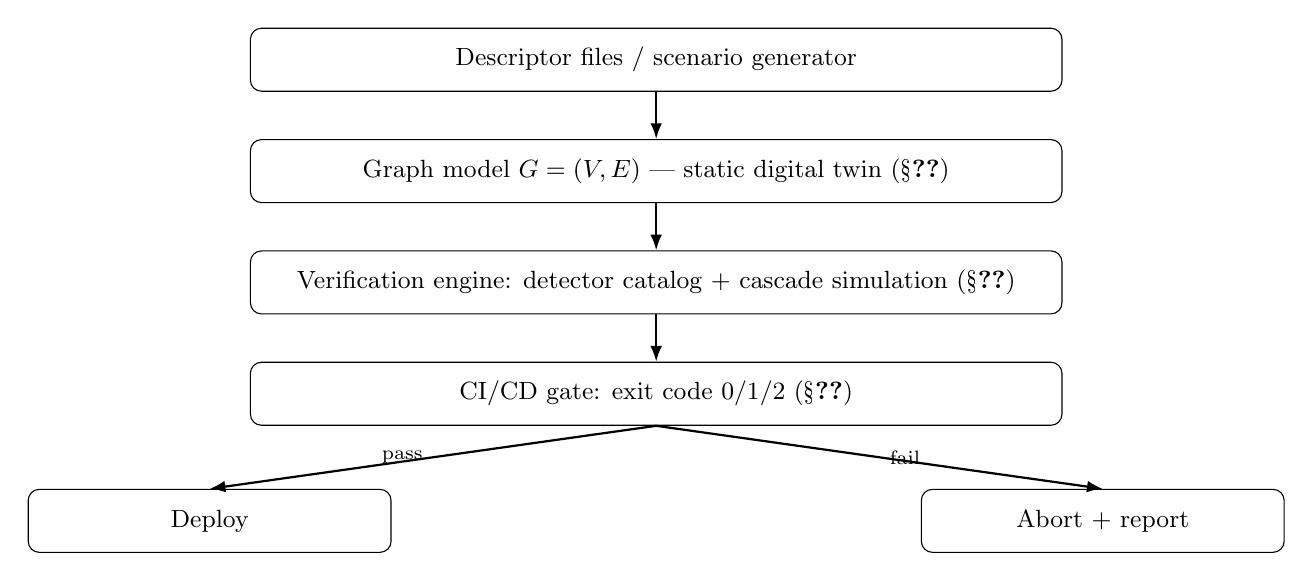
\begin{tikzpicture}[
    node distance=6mm,
    box/.style={draw, rounded corners, align=center, minimum width=0.85\linewidth, minimum height=8mm, font=\small},
    arr/.style={-{Latex[length=2mm]}, thick}
  ]
  \node[box] (src) {Descriptor files / scenario generator};
  \node[box, below=of src] (graph) {Graph model $G=(V,E)$ --- static digital twin (\S\ref{sec:graphmodel})};
  \node[box, below=of graph] (ver) {Verification engine: detector catalog + cascade simulation (\S\ref{sec:verification})};
  \node[box, below=of ver] (gate) {CI/CD gate: exit code 0/1/2 (\S\ref{sec:gating})};
  \node[box, below left=8mm and -18mm of gate, minimum width=0.38\linewidth] (deploy) {Deploy};
  \node[box, below right=8mm and -18mm of gate, minimum width=0.38\linewidth] (abort) {Abort + report};
  \draw[arr] (src) -- (graph);
  \draw[arr] (graph) -- (ver);
  \draw[arr] (ver) -- (gate);
  \draw[arr] (gate.south) -- node[left,font=\scriptsize] {pass} (deploy.north);
  \draw[arr] (gate.south) -- node[right,font=\scriptsize] {fail} (abort.north);
\end{tikzpicture}
\caption{SaaG pipeline overview. The graph (SaaG-P's static twin) is rebuilt per candidate build
(\S\ref{sec:isolation}) and audited before the gate decision; SaaG-D specifies a scored variant of
the same gate (\S\ref{sec:scoringmodel}) not yet built in the prototype.}
\label{fig:architecture}
\end{figure}

\section{Verification Engine}
\label{sec:verification}

\subsection{What the Prototype Checks Today}
\label{sec:checks}

SaaG-P implements a catalog of structural and criticality-weighted detectors over the derived
dependency graph. Those bearing directly on the defect classes of \S\ref{sec:gap}:

\begin{itemize}
\item \textbf{Orphaned topics} --- publishers with no subscribers or vice versa, the structural
  signature of the refactor in \S\ref{sec:gap}.
\item \textbf{Dependency cycles} --- strongly connected components over the application dependency
  subgraph.
\item \textbf{SPOFs and bottlenecks} --- articulation points and bridge edges, ranked by
  propagated QoS weight.
\item \textbf{Structural concentration} --- broker overload, topic fan-out, hub-and-spoke
  concentration, deep pipelines, god components.
\end{itemize}

Detectors emit findings with a severity (CRITICAL/HIGH/MEDIUM), affected components, the rule
that fired, and a recommendation.

\subsection{Cascade Impact Simulation}
\label{sec:cascade}

Beyond static rules, SaaG-P simulates component failure to estimate blast radius before
deployment. Failure is injected at a component and propagated along structural pub/sub
edges --- never along the derived \texttt{DEPENDS\_ON} edges, an independence property enforced by
the prototype's test suite so that simulation cannot silently consume its own derived output. The
result ranks components by cascade impact, which is what \S\ref{sec:prototype} uses as a reference
oracle when scoring the detector catalog.

\subsection{Scenario Generation}
\label{sec:scenariogen}

Verification requires system models that do not yet exist in the field. SaaG-P includes a scenario
generator producing synthetic topologies with controlled scale, QoS mix, and clustering, plus a
curated corpus of fifteen committed scenarios: ten spanning autonomous vehicles, IoT, financial
trading, healthcare, and enterprise deployments at various scales, plus --- the evaluation's primary
focus, \S\ref{sec:prototype} --- a five-scenario family in the air-traffic-management domain that
mirrors the deployment motivating this paper (\S\ref{sec:msd}), spanning 29 to 444 components and
sharing an identical QoS-mix, fan-out-shape, and criticality-proportion profile so that scale is
the only thing that varies between them. Each is hash-pinned against the config that generates it,
so published numbers remain reproducible. Three architectures transcribed from open-source systems
(\S\ref{sec:external-validity}) share the same descriptor schema and load through the identical
pipeline, letting the secondary evaluation compare generated and transcribed topologies directly
rather than describing the latter only qualitatively.

\subsection{Specified but Not Yet Implemented}
\label{sec:gap-table}

The following are required of SaaG-D and are \textbf{not} implemented in SaaG-P. We list them
because the gap is the most transferable finding in this paper: each is a check whose value is
obvious and whose cost is dominated by acquiring a domain model the graph does not carry.

\begin{table*}[t]
\caption{Specified capabilities not yet implemented in SaaG-P. None are blocked on graph
technology; four of the seven are blocked on input acquisition (\S\ref{sec:gap-table}).}
\label{tab:gaptable}
\footnotesize
\begin{tabular}{@{}p{0.30\linewidth}p{0.62\linewidth}@{}}
\toprule
\textbf{Capability} & \textbf{Why it is not yet built} \\
\midrule
\textbf{QoS contract conformance} --- request/offer matching of durability, reliability, transport
priority per topic &
Flags a criticality-gap \emph{anomaly}, not a contract violation: needs per-endpoint QoS at
reader/writer granularity; the model currently attaches QoS to the topic. \\
\textbf{Payload schema consistency} --- same topic name, divergent content definition &
Requires parsing/comparing IDL/message definitions across units; the extractor does not yet
resolve type definitions. \\
\textbf{Core allocation conformance} --- capacity, conflicting pinning, dedicated high-performance
cores &
Core/memory sizes are node attributes but no rule evaluates them; needs core-assignment
descriptors outside the prototype's inputs. \\
\textbf{OS and runtime configuration audit} --- OS settings vs.\ allocation &
Same cause: not in the prototype's input set. \\
\textbf{Architectural drift} --- designed vs.\ observed topology (the dynamic half of the digital
twin, \S\ref{sec:twoartifacts}) &
Needs a field-record store and a graph-diff over observed edges; neither exists in the prototype. \\
\textbf{Installation suitability scoring} --- four headings, per-rule weights, blocking flags,
aggregate score &
The gate is severity-based, not score-based (\S\ref{sec:gating}); specified in
\S\ref{sec:scoringmodel} as a requirement, not a result. \\
\textbf{CMDB and network topology ingestion} &
Prototype consumes descriptor files instead. \\
\bottomrule
\end{tabular}
\end{table*}

Note what the table does \emph{not} say: none of these are blocked on graph technology. Four of the
seven are blocked on \textbf{input acquisition} --- the information exists in the program but not in
a form the model ingests. That ratio is our main lesson for teams attempting the same thing.

\section{CI/CD Gating}
\label{sec:gating}

\begin{figure*}[t]
\centering
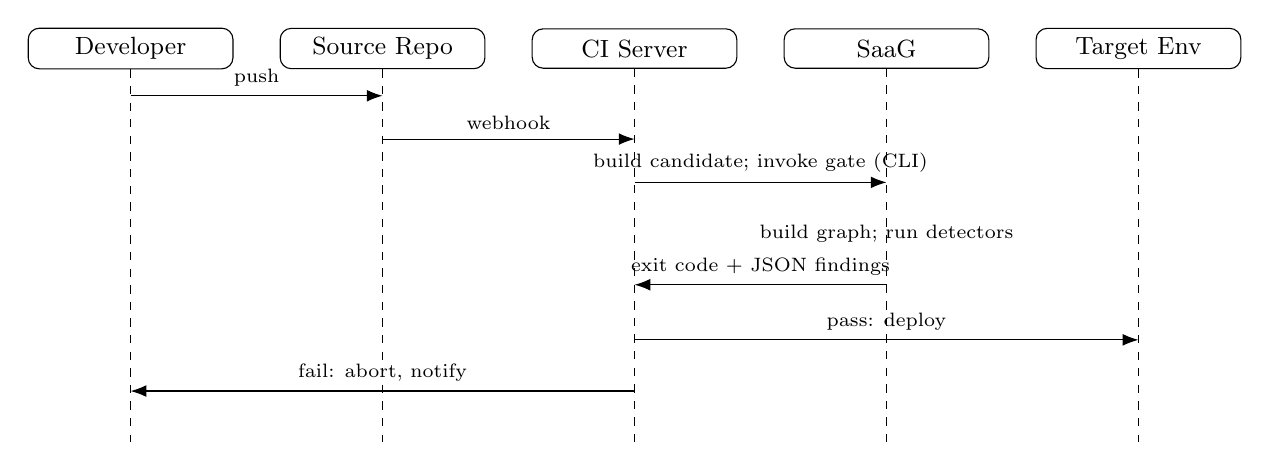
\begin{tikzpicture}[
    font=\small,
    actor/.style={draw, rounded corners, align=center, minimum width=2.6cm, minimum height=5mm},
    lifeline/.style={dashed},
    msg/.style={-{Latex[length=2mm]}, font=\scriptsize}
  ]
  \def\actorY{0}
  \def\lifelineBottom{-5.0}
  \foreach \name/\lbl/\x in {dev/{Developer}/0, repo/{Source Repo}/3.2, ci/{CI Server}/6.4,
                                 saag/{SaaG}/9.6, target/{Target Env}/12.8} {
    \node[actor] (\name) at (\x, \actorY) {\lbl};
    \draw[lifeline] (\name.south) -- (\x, \lifelineBottom);
  }
  \draw[msg] (dev.south |- 0,-0.6) -- node[above]{push} (repo.south |- 0,-0.6);
  \draw[msg] (repo.south |- 0,-1.15) -- node[above]{webhook} (ci.south |- 0,-1.15);
  \draw[msg] (ci.south |- 0,-1.7) -- node[above,align=center]{build candidate; invoke gate (CLI)} (saag.south |- 0,-1.7);
  \node[font=\scriptsize] at (9.6,-2.35) {build graph; run detectors};
  \draw[msg] (saag.south |- 0,-3.0) -- node[above,align=center]{exit code + JSON findings} (ci.south |- 0,-3.0);
  \draw[msg] (ci.south |- 0,-3.7) -- node[above]{pass: deploy} (target.south |- 0,-3.7);
  \draw[msg] (ci.south |- 0,-4.35) -- node[above]{fail: abort, notify} (dev.south |- 0,-4.35);
\end{tikzpicture}
\caption{Gate integration sequence. The prototype's decision is the process exit code
(\S\ref{sec:implgate}).}
\label{fig:sequence}
\end{figure*}

\subsection{The Implemented Gate}
\label{sec:implgate}

SaaG-P integrates as a command-line invocation. It constructs the candidate graph, runs the
detectors, optionally writes the full finding set as JSON for downstream tooling, and encodes its
decision in the process exit status: \textbf{2} if any CRITICAL or HIGH finding is present,
\textbf{1} if any finding is present, \textbf{0} if none. Standard CI runners treat non-zero as
failure, so a two-line pipeline stage gets absolute severity gating with no plugin
(Figure~\ref{fig:sequence}).

Two limitations are worth stating because they are the difference between a usable gate and a
tolerated one:

\begin{itemize}
\item \textbf{The gate is absolute, not delta-aware.} It scores the candidate graph on its own,
  not against the merge base, so a codebase carrying pre-existing HIGH findings fails every build
  until cleared --- in practice, teams disable the gate. Not hypothetical here: at CRITICAL/HIGH
  severity, \textbf{all sixteen systems we evaluated} (five ATM scale points,
  \S\ref{sec:cost-atm}--\S\ref{sec:catalog-atm}; eleven secondary-corpus scenarios,
  \S\ref{sec:external-validity}) \textbf{return exit code 2 at every oracle seed tested} --- exactly
  the failure mode that gets a gate disabled rather than heeded. Delta semantics and a waiver
  register are the first changes we would make; a learned, delta-aware, simulation-verified gate is
  the companion manuscript's~\cite{companion2026} contribution, cited here as the direction rather
  than duplicated.
\item \textbf{There is no severity budget.} One HIGH finding and three hundred are the same
  decision.
\end{itemize}

\subsection{The Specified Scoring Model}
\label{sec:scoringmodel}

SaaG-D is specified to replace the exit-code gate with a scored evaluation over four
headings --- structural/architectural, interface/topic/communication, dependency/integration, and
resource/performance conformance. Each rule carries an identifier, heading, severity, weight,
acceptance criterion, and blocking flag. A finding at critical severity, or a blocking-rule
violation, yields a non-conforming decision \textbf{independently of the aggregate score} --- the
score is for reporting and trend analysis; blocking is categorical. Multi-unit evaluations run
under independent operation identifiers, returning per-unit decisions plus an aggregate result in
machine-processable form.

We report this as specification, not as measurement: it is not implemented in SaaG-P, and
\S\ref{sec:evaluation} makes no claim about its behaviour.

\subsection{Findings and Reports}
\label{sec:findings}

Each finding carries an identifier, type, description, affected entity, the rule or acceptance
criterion it derives from, supporting evidence, and a severity level. This evidence-bearing
structure is what makes a failing gate actionable rather than merely obstructive: the developer
receives the offending component and the rule, not a build log.

\section{Evaluation}
\label{sec:evaluation}

Two evaluations, kept separate. \S\ref{sec:deployment} reports the deployment ([I]);
\S\ref{sec:prototype} reports the open prototype ([P]) and is fully reproducible. Neither
substitutes for the other: the deployment numbers describe real engineering impact but cannot be
independently verified; the prototype numbers can be rerun by any reader but describe a subset of
the capability.

\subsection{Deployment Experience [I] --- TODO(data)}
\label{sec:deployment}

\textbf{Status: awaiting cleared data.} Every figure below must carry an $n$, a window, and
provenance, and appear only where the corresponding check actually ran in the deployment; this
subsection is not written until the underlying data is filled in, so no placeholder numbers appear
in this draft: system scale at the audited baseline; per-stage verification wall-clock against
build time; defects caught before deployment by category, with confirmation status where tracked;
and production incidents before/after gating, normalized per release, with confounders listed
explicitly rather than a bare percentage drop.

\subsection{Prototype Measurements [P]}
\label{sec:prototype}

Two studies. The \textbf{primary study} (\S\ref{sec:cost-atm}--\S\ref{sec:catalog-atm}) evaluates a
family of five systems in the deployment's own domain --- air traffic management --- at five scales,
regenerating from a single committed artifact produced by an automated seed sweep. The
\textbf{secondary study} (\S\ref{sec:external-validity}), carried forward unchanged from the prior
revision, checks whether the primary study's pattern generalizes across \emph{other} domains
rather than across scale within one.

The primary study's five systems --- 29, 74 (the original \texttt{atm\_system} scenario, unchanged),
148, 296, and 444 components --- are generated from configs that hold QoS mix, fan-out shape, and
criticality proportion identical across scales and vary only entity counts, so \textbf{scale is
the sole independent variable} --- an improvement on the secondary study's corpus, where domain and
scale changed together and could not be separated. Each of the five is evaluated at five oracle
seeds ($\{42, 123, 456, 789, 2024\}$), 25 runs total, zero failures.

\subsubsection{Verification Cost by ATM Scale}
\label{sec:cost-atm}

End-to-end cost of one gate invocation --- graph analysis plus all detectors --- against component
count, domain held fixed, mean $\pm$ std over the five seeds:

\begin{table}[t]
\caption{Gate cost by ATM scale, mean $\pm$ std over 5 oracle seeds, layer = system.}
\label{tab:cost}
\footnotesize
\begin{tabular}{@{}lrrrr@{}}
\toprule
\textbf{Scale} & \textbf{Comp.} & \textbf{Analysis (s)} & \textbf{Detect (s)} & \textbf{Gate (s)} \\
\midrule
tiny             & 29  & $0.01\pm0.00$ & $0.00\pm0.00$ & $0.01\pm0.00$ \\
small (\texttt{atm\_system}) & 74  & $0.05\pm0.00$ & $0.00\pm0.00$ & $0.05\pm0.00$ \\
medium           & 148 & $0.13\pm0.00$ & $0.00\pm0.00$ & $0.13\pm0.00$ \\
large            & 296 & $0.52\pm0.02$ & $0.01\pm0.00$ & $0.53\pm0.02$ \\
xlarge           & 444 & $0.99\pm0.03$ & $0.02\pm0.00$ & $1.01\pm0.03$ \\
\bottomrule
\end{tabular}
\end{table}

Two observations. First, \textbf{detection is cheap here too, more so than the secondary corpus}:
even at 444 components the full detector suite costs 0.02\,s, and summed across all five scales the
costliest single detector (cycle detection) averages 0.005\,s --- cheaper than the secondary
corpus's already-cheap 0.047\,s (\S\ref{sec:external-validity}), because this domain's fixed
fan-out shape keeps the dependency graph sparse at every scale.

Second, \textbf{this controlled sweep resolves an ambiguity the secondary corpus left open.}
There, analysis cost jumped sharply between 326 and 520 components (a 25$\times$ increase for a
1.6$\times$ size increase), and it was unclear whether that reflected component count or the
specific topology of that one 520-component scenario. Here, holding domain and topology shape
fixed and scaling components alone from 29 to 444 (a 15$\times$ increase) produces a
\textbf{roughly proportional} cost increase --- 0.01\,s to 0.99\,s, about 100$\times$ --- with no
cliff. The secondary corpus's steep jump was therefore a property of that one scenario's structure
(or, per its own wall-clock caveat, of host load at measurement time), not a general law that cost
explodes past a few hundred components. For this paper's motivating domain, at least, cost growth
is gentle.

\subsubsection{Detector Catalog Against a Cascade Oracle, by ATM Scale}
\label{sec:catalog-atm}

We scored the catalog's flagged set against the oracle's critical set --- box-plot top tier
($\ge Q_3$) once a scale has enough scored components to estimate quartiles, a top-20\% mask below
that, the same rule applied elsewhere in this codebase --- at each of the five scales. Unlike
\S\ref{sec:cost-atm}'s cost measurement, this result is a genuine trend across scale rather than a
single robustness check, so we report one row per scale instead of pooling:

\begin{table}[t]
\caption{Rule-based detection vs.\ simulated cascade impact, by ATM scale. ``Seed-inv.'' scales
report a single value (all 5 seeds bit-identical); xlarge --- the one exception --- reports
mean $\pm$ std (4 of 5 seeds agree exactly; one seed's critical set differs by a single
component).}
\label{tab:catalog}
\tiny
\setlength{\tabcolsep}{2pt}
\begin{tabular}{@{}lrrrrrrc@{}}
\toprule
\textbf{Scale} & \textbf{Comp.} & \textbf{Prec.} & \textbf{Rec.} & \textbf{$F_1$} &
\textbf{$\kappa$} & \textbf{\%flag} & \textbf{S.I.} \\
\midrule
tiny   & 29  & 0.250 & 1.000 & 0.400 & 0.118 & 80.0\% & Y \\
small  & 74  & 0.273 & 0.900 & 0.419 & 0.041 & 84.6\% & Y \\
medium & 148 & 0.269 & 0.900 & 0.414 & 0.031 & 85.9\% & Y \\
large  & 296 & 0.250 & 0.949 & 0.396 & 0.000 & 94.9\% & Y \\
xlarge & 444 & $0.235{\pm}.002$ & $0.868{\pm}.007$ & $0.370{\pm}.003$ & $-0.045{\pm}.005$ & 93.2\% & N \\
\bottomrule
\end{tabular}
\end{table}

\textbf{Agreement declines monotonically as the same ATM system grows}, from $\kappa = 0.118$
(slight agreement) at 29 components to $\kappa \approx -0.045$ (no better than chance) at 444,
crossing zero at the 296-component point. The mechanism is visible in the same table: the fraction
of scored components the catalog flags climbs from 80.0\% to 93--95\% as scale increases, so
precision erodes steadily (0.273 $\rightarrow$ 0.235) while recall stays high throughout
(0.868--1.000). This is the same over-flagging mechanism identified in the secondary corpus
(\S\ref{sec:external-validity}) --- but here it is a genuine trend \emph{within} one domain rather
than a difference \emph{between} domains: \textbf{as this ATM family grows, findings volume stays
cheap to compute (\S\ref{sec:cost-atm}), but the catalog gets steadily less discriminating.}

\textbf{This is a mechanical consequence of how the catalog verdict is built, not evidence it
fails to find critical components.} Unlike the RM composite score $Q(v)$, threshold-matched to
the oracle's critical-set size on both sides so precision/recall converge by construction, the
catalog is a binary ``flagged by at least one rule'' decision whose flagged fraction is whatever
the rule union produces, not a calibrated boundary:
$\text{precision} = \text{base\_rate} \times \text{recall} \, / \, \text{flagged\_fraction}$
reproduces the measured precision to three decimals at every scale (xlarge:
$0.252 \times 0.864 / 0.932 = 0.234$, measured $0.235$), so \textbf{$F_1$'s trend is just the
flagged-fraction trend read backwards}, not a failure to detect --- recall never drops below 0.868.
We read the \emph{decline itself} more cautiously, since the generator recycles the same six roles
at every scale rather than adding subsystems (\S\ref{sec:threats}).

\subsubsection{External Validity: Generality Beyond ATM}
\label{sec:external-validity}

The primary study asks whether verification quality holds as \emph{one} domain scales. A separate
question --- does a pattern found on one domain generalize to \emph{other} domains? --- was the
focus of the prior revision's evaluation, retained here as a secondary check. It used eight
generated scenarios spanning six other domains (29 to 520 components, domain and scale varying
together) plus three architectures transcribed from open-source systems (Autoware.universe ROS~2,
the Train-Ticket microservices benchmark, and a cloud-native microservices mesh; 60--90
components), at the same five oracle seeds:

\begin{table}[t]
\caption{Rule-based detection vs.\ simulated cascade impact, cross-domain secondary corpus
(unchanged from the prior revision).}
\label{tab:secondary}
\tiny
\setlength{\tabcolsep}{2pt}
\begin{tabular}{@{}lrrrrrr@{}}
\toprule
\textbf{Corpus} & \textbf{$n$} & \textbf{Prec.} & \textbf{Rec.} & \textbf{$F_1$} &
\textbf{$\kappa$} & \textbf{\%flag} \\
\midrule
Generated (6 domains) & 8 & $0.237{\pm}.015$ & $0.887{\pm}.063$ & $0.374{\pm}.023$ &
$-0.036{\pm}.053$ & 93.7\% \\
Transcribed (real) & 3 & $0.402{\pm}.073$ & $0.865{\pm}.126$ & $0.546{\pm}.077$ &
$0.299{\pm}.126$ & 56.3\% \\
\bottomrule
\end{tabular}
\end{table}

Agreement on the six other generated domains was near-chance ($\kappa \approx 0$), matching this
paper's ATM finding at large scale, but agreement on the three \emph{transcribed, real}
architectures was materially better (fair, $\kappa \approx 0.30$), driven by less over-flagging
(56.3\% vs.\ 93.7--94.9\%) --- the same mechanical identity from \S\ref{sec:catalog-atm} applies
here too. The pattern that best fits the evidence: \textbf{rule-based flagging is least
discriminating on large, synthetically-generated graphs regardless of domain, and more
discriminating on smaller and/or non-synthetic ones} --- but scale and ``generated-ness'' point the
same direction here, so this corpus cannot cleanly separate which drives the effect. Caveats
restated in \S\ref{sec:threats}.

\subsection{Threats to Validity}
\label{sec:threats}

\begin{itemize}
\item \textbf{Two systems, one name.} \S\ref{sec:deployment} and \S\ref{sec:prototype} measure
  different artifacts (\S\ref{sec:twoartifacts}). The prototype implements a subset of the
  deployed capability; prototype cost figures are lower bounds on deployed cost.
\item \textbf{Simulated oracle.} \S\ref{sec:catalog-atm} and \S\ref{sec:external-validity} score
  detection against a simulator, not against observed field failures. The simulator is a model of
  cascade propagation, and agreement with it is not the same as agreement with reality. A second
  independent oracle in the same codebase agrees with this one at only $\rho \approx 0.40$, which
  bounds how far any figure measured on one transfers to the other.
\item \textbf{Same six roles, recycled, not new subsystems.} The ATM generator's domain skin
  (\S\ref{sec:gap-table}) supplies six named roles and a fixed five-cluster hierarchy regardless of
  scale --- growing from 29 to 444 components means more copies of the same six roles, not new
  subsystem types, which may not resemble how a real deployment adds capacity.
\item \textbf{Effective sample size is 5 scale points, not 25 scale-seed pairs.} Four of five are
  seed-confirmed exactly, the fifth to within std $\le 0.005$: this rules out a lucky seed, but one
  generator draw per scale is one trajectory, not several independent ones.
\item \textbf{Corpus composition.} The primary study is entirely single-domain and synthetic. The
  only cross-domain, partially non-synthetic evidence is the secondary corpus
  (\S\ref{sec:external-validity}): $n=8$/$n=3$, seed-invariant for 10 of 11 scenarios, a $2\times$
  wall-clock discrepancy against an earlier measurement, and hand-built (not harvested)
  transcriptions.
\item \textbf{Confounders.} Gating was not the only change in \S\ref{sec:deployment}'s
  production-incident observation window; listed confounders bound the causal claim.
\end{itemize}

\section{Related Work}
\label{sec:relatedwork}

\textbf{Architecture description languages.} AADL and SysML model hardware/software interaction
and support analysis of the same properties we target~\cite{feilergluch2012}, but the model is
authored separately from the implementation and drifts. SaaG's model is reconstructed per
candidate build from artifacts the build already produces, trading expressiveness for currency.

\textbf{Static code analysis and runtime observability.} SonarQube and Coverity analyze source and
local control flow, structurally unable to see topic bindings, QoS contracts, or node topology
since the system exists only in the composition of individually-analyzed units. Observability
platforms (Prometheus, Dynatrace) see the deployed system with fidelity no static model matches,
but only after a non-conforming artifact is already running. SaaG complements the former at the
architectural boundary and, through the specified drift detection of \S\ref{sec:gap-table}, aims
to route the latter's kind of observation back into pre-deployment verification.

\textbf{Digital twins.} The term is established in manufacturing and Industry~4.0, where a digital
twin synchronizes a model against a physical asset via continuous sensor
telemetry~\cite{tao2019}. The object and fidelity are both different here: the twin models a
\emph{software architecture}, not a physical asset, and is \emph{static} (\S\ref{sec:twoartifacts}),
reconstructed per candidate build rather than continuously live. We use the term because the
reconstruct-and-audit pattern is the same one digital-twin systems apply to physical assets, and
the specified, not-yet-built dynamic half (\S\ref{sec:gap-table}) is exactly the
telemetry-synchronization step the literature describes; we do not claim a live-synchronized model
we have not built.

\textbf{Middleware dependability.} Pub/sub dependability has been studied at the protocol, broker
overlay, and runtime levels~\cite{eugster2003,carzaniga2001}. Our contribution is neither a
protocol nor a runtime mechanism but a pipeline-integrated static check over the deployment's own
descriptors.

% TODO(refs): expand from 9 to ~18 citations before submission -- see refs.bib header comment.

\section{Conclusion}
\label{sec:conclusion}

We reported an architectural digital twin, a requirements baseline, an open prototype, and a
CI/CD gate, with measurements from both an industrial deployment and the prototype
(\S\ref{sec:contrib}). The findings we would most want carried forward are the negative ones, plus
one that surprised us. Building the graph and running structural rules is cheap regardless of
scale (\S\ref{sec:cost-atm}), but ranking findings by consequence gets worse as the same system
grows: rule-based severity agrees with simulated cascade impact at $\kappa = 0.12$ (slight) on the
smallest ATM system and $\kappa \approx -0.05$ (chance) on the largest --- same domain, same
generator template, only scale different (\S\ref{sec:catalog-atm}). A secondary check found the
same near-chance pattern on other synthetic domains but materially better agreement on transcribed
real architectures (\S\ref{sec:external-validity}); scale and synthetic generation both point
toward the failure mode, and this paper's evidence cannot separate which is the true cause. Four of
the seven specified checks we have not built are blocked not on analysis technique but on
\textbf{getting configuration data into the model at all} (\S\ref{sec:gap-table}): budget for data
acquisition, not graph algorithms.

\textbf{Future work.} Delta-aware gating with a waiver register (\S\ref{sec:implgate});
reader/writer-granularity QoS conformance (\S\ref{sec:gap-table}); drift detection via the
specified field-record path; and, highest priority, confirming the within-domain $\kappa$ decline
against a real, growing deployment rather than a synthetic scale sweep of one generator template.

\bibliographystyle{ACM-Reference-Format}
\bibliography{refs}

\end{document}
